\title{\textbf{Squeezing Heads: Head-Aware Knowledge Distillation via LoRA-Wrapped Attention}

\author{Anonymous authors}



\section{Introduction}

\subsection{Motivation}

Multi-head self-attention is the core operation of every modern transformer, 
but it is also the largest consumer of parameters and compute. A standard 
12-layer BERT-base model has 12 attention heads per layer, each with its own 
$W_Q, W_K, W_V, W_O$ projections totaling 4.7M parameters per layer.

\textbf{Head redundancy is well documented.} Voita et al. (2019) find that over 
half of the heads in BERT can be pruned without significant accuracy loss. 
Michel et al. (2019) show that in many layers, a \textbf{single head} is 
sufficient. Clark et al. (2019) characterize attention patterns as 
"positional", "syntactic", or "rare-word" -- with the majority falling into 
redundant categories.

\textbf{The naive approach -- prune heads -- loses information.} Simply removing 
a head discards whatever information it carried. If the head was doing 
something useful, accuracy drops.

\textbf{The alternative -- fine-tune the full model -- is expensive.} Retraining a 
pruned model requires substantial compute and full-parameter optimization.

\textbf{The opportunity.} What if we could \textbf{wrap} the pretrained attention with 
a small trainable adapter, and let the adapter learn to compensate for 
compressed head capacity? This is the idea behind \textbf{Squeezing Heads}.

\subsection{Problem Statement}

Given a pretrained transformer with $H$ attention heads per layer, we seek 
a modified module $\mathcal{A}'$ such that:

\begin{enumerate}
\item \textbf{Compressible:} Effective head dimension can be reduced by a factor $s$.
\item \textbf{Distillable:} Trainable adapters can recover lost capacity.
\item \textbf{Drop-in:} Pretrained weights are copied exactly; no architecture change.
\item \textbf{Portable:} Works across flat, nested, and causal architectures.
\item \textbf{Quality:} $\Delta\text{Acc} \leq 5\%$ on SST-2.

\end{enumerate}
\subsection{Our Approach: Squeezing Heads}

\textbf{Squeezing Heads} replaces each attention projection with a 
\textbf{LoRA-wrapped linear layer}:

\begin{equation}
W_\text{eff} = W_\text{frozen} + \frac{\alpha}{r} B A
\end{equation}

where:
\begin{itemize}
\item $W_\text{frozen}$ is the pretrained projection (unchanged).
\item $B A$ is a low-rank adapter with rank $r$ (trainable).
\item $\alpha$ is the LoRA scaling factor.

\end{itemize}
\textbf{Figure 1.1} compares three head-compression strategies:

\begin{table}[H]
\centering
\small
\begin{tabular}{llll}
\toprule
\textbf{Strategy} & \textbf{Prunes heads?} & \textbf{Trains full model?} & \textbf{Recovers info?} \\
\midrule
Head pruning \& Yes \& No &  \\
Full fine-tune \& Yes \& Yes & (expensive) \\
\textbf{Squeezing Heads} \& Optional & \textbf{LoRA only} &  \\
\bottomrule
\end{tabular}
\end{table}

\textbf{Key design choices:}

\begin{enumerate}
\item \textbf{Wrapper, not replacement.} The pretrained attention is preserved
  exactly. Only the LoRA parameters differ from initialization.
\item \textbf{Per-projection LoRA.} Each of $W_Q, W_K, W_V, W_O$ has its own LoRA
  adapter, allowing fine-grained capacity allocation.
\item \textbf{GQA-aware pooling.} When the source model uses GQA (Qwen, LLaMA),
  we pool the source KV heads into the target head count.
\item \textbf{Principal head preservation.} When the head dimension is reduced, we
  preserve the leading head dimensions (the principal components) rather
  than random slices.

\end{enumerate}
\subsection{Contributions}

\begin{itemize}
\item \textbf{A LoRA-wrapped attention for head distillation.} Squeezing Heads
  preserves pretrained weights exactly while enabling low-rank adaptation.
\item \textbf{A GQA-aware copy procedure.} We handle the Grouped Query Attention
  case by pooling source KV heads.
\item \textbf{Multi-architecture support.} DistilBERT, RoBERTa, GPT-2, and Qwen with
  RoPE, GQA, and causal masking preserved.
\item \textbf{A systematic evaluation.} Benchmarked on DistilBERT, RoBERTa, and GPT-2
  on SST-2 with ablations over LoRA rank, head-dim reduction, and GQA
  pooling.
\item \textbf{Full reproducibility.} Code, checkpoints, and evaluation scripts
  released under MIT.

\end{itemize}
\subsection{Paper Organization}

Section 2 reviews related work. Section 3 provides background on attention, 
LoRA, and head pruning. Section 4 presents Squeezing Heads. Section 5 
describes integration with four architectures. Section 6 details the 
experimental setup. Section 7 reports results. Section 8 analyzes the 
contribution of LoRA and head-dim reduction. Section 9 discusses practical 
guidance. Section 10 lists limitations. Section 11 concludes.



\subsection{Notation}

\begin{lstlisting}

---
\end{lstlisting}


\section{Related Work}

\subsection{Head Pruning}

\textbf{Voita et al. (2019):} Layer-wise relevance propagation to rank heads. 
Prune 38 heads (of 48) in BERT with small loss.

\textbf{Michel et al. (2019):} Show that a single head suffices for many tasks. 
Gradient-based importance.

\textbf{Clark et al. (2019):} Analyze attention patterns. Categorize heads as 
positional, syntactic, rare-word, or non-specialized.

\textbf{Squeezing Heads differs} by \textbf{not pruning} -- instead, all heads are 
kept but their dimensionality is reduced, and LoRA adapters learn to 
compensate.

\subsection{Knowledge Distillation}

\textbf{Hinton et al. (2015):} Original KD. Train a small student to match a 
large teacher's logits.

\textbf{DistilBERT (Sanh et al., 2019):} Distill BERT into 6 layers with soft 
targets and cosine loss.

\textbf{TinyBERT (Jiao et al., 2020):} Distill both logits and hidden states.

\textbf{Squeezing Heads is orthogonal} -- it can be combined with any of these.

\subsection{Parameter-Efficient Fine-Tuning}

\textbf{LoRA (Hu et al., 2021):} Freeze base weights, add rank-$r$ adapters.

\textbf{AdaLoRA (Zhang et al., 2023):} Adaptive rank allocation.

\textbf{DoRA (Liu et al., 2024):} Magnitude-direction decomposition.

\textbf{Squeezing Heads uses LoRA} as the recovery mechanism.

\subsection{Attention Distillation}

\textbf{TinyBERT:} Attention transfer loss.

\textbf{MiniLM (Wang et al., 2020):} Self-attention distillation.

\textbf{Squeezing Heads differs} by using LoRA adapters as the distillation 
target -- the objective is on the wrapped attention, not on logits.

\subsection{Position of Our Work}

\begin{table}[H]
\centering
\small
\begin{tabular}{lllll}
\toprule
\textbf{Axis} & \textbf{Head Pruning} & \textbf{KD} & \textbf{LoRA} & \textbf{Squeezing Heads} \\
\midrule
Preserves all heads &  &  & -- &  \\
Trains LoRA only &  &  &  &  \\
Multi-architecture \& Varies &  &  &  \\
GQA-aware &  &  &  &  \\
\bottomrule
\end{tabular}
\end{table}

\subsection{Comparison Table}

\begin{lstlisting}

---
\end{lstlisting}


\section{Background}

\subsection{Multi-Head Self-Attention}

For input $X \in \mathbb{R}^{B \times L \times d}$:

\begin{equation}
Q = X W_Q, \quad K = X W_K, \quad V = X W_V
\end{equation}

\begin{equation}
\text{head}_h = \text{softmax}\!\left(\frac{Q_h K_h^\top}{\sqrt{d_h}}\right) V_h
\end{equation}

\begin{equation}
\text{MHSA}(X) = \text{Concat}(\text{head}_1, \dots, \text{head}_H) W_O
\end{equation}

\textbf{Parameter count.} $W_Q, W_K, W_V \in \mathbb{R}^{d \times d}$, 
$W_O \in \mathbb{R}^{d \times d}$. Total: $4 d^2$.

\subsection{Head Redundancy}

Empirical findings:

\begin{itemize}
\item Most heads in BERT can be pruned (Voita et al., 2019).
\item Many layers need only one head (Michel et al., 2019).
\item Head patterns are dominated by a few categories (Clark et al., 2019).

\end{itemize}
\textbf{Implication.} Reducing head capacity is a viable compression strategy.

\subsection{LoRA}

LoRA (Hu et al., 2021) parameterizes weight updates as:

\begin{equation}
W_\text{eff} = W_\text{frozen} + \frac{\alpha}{r_L} B A
\end{equation}

where $A \in \mathbb{R}^{r_L \times d}$, $B \in \mathbb{R}^{d \times r_L}$, 
$B = 0$ at initialization. Only $A, B$ are trained.

\textbf{Benefits.}
\begin{itemize}
\item \textbf{Small trainable footprint:} $2 r_L d$ vs $d^2$.
\item \textbf{Preserves pretrained:} Base weights unchanged.
\item \textbf{Composable:} Multiple LoRA adapters can be combined.

\end{itemize}
\subsection{Grouped Query Attention (GQA)}

GQA (Ainslie et al., 2023) uses $H_{kv} < H$ KV heads. When the source 
attention has more heads than the target, we pool:

\begin{equation}
W_K^{(\text{target})}_g = \frac{1}{r} \sum_{h \in g} W_K^{(\text{source})}_h
\end{equation}

where $r = H_\text{source} / H_\text{target}$.

\subsection{Rotary Position Embeddings (RoPE)}

RoPE (Su et al., 2021) applies position-dependent rotation:

\begin{equation}
\tilde{Q}_i = Q_i \cos(\theta_i) + \text{rot}(Q_i) \sin(\theta_i)
\end{equation}

Squeezing Heads preserves RoPE through the wrapper.

\subsection{Head Dimension Reduction}

When reducing head dimension from $d_h$ to $d_h / s$:

\begin{equation}
W_Q^{(\text{new})} = W_Q^{(\text{old})}_{:d_h/s, :}
\end{equation}

We preserve the \textbf{leading} $d_h / s$ rows, corresponding to the principal 
components of the head.

\subsection{Notation Summary}

\begin{lstlisting}

---
\end{lstlisting}


\section{Method}

\subsection{Overview}

Squeezing Heads replaces each pretrained attention projection with a 
\textbf{LoRA-wrapped linear layer}:

\begin{equation}
\text{Projection}_{W} = \text{LoRALinear}(W_\text{frozen}, r_L, \alpha)
\end{equation}

The forward pass is:

\begin{equation}
y = x W_\text{frozen}^\top + \frac{\alpha}{r_L} x A^\top B^\top + b
\end{equation}

where $W_\text{frozen}$ is the pretrained weight (frozen), $A, B$ are LoRA 
adapters (trainable), and $b$ is the bias (frozen).

\textbf{Figure 4.1} illustrates the pipeline.

\begin{lstlisting}
    Input X
       |
       +--------------------+
                             
  +----------+        +----------+
  | Frozen   |        | LoRA     |
  | W_frozen |        | BA       |
  +----+-----+        +----+-----+
       |                   |
       +---------+---------+
                  
           y = Wx + ($\alpha$/r)BAx + b
\end{lstlisting}

\subsection{LoRA-Wrapped Projection}

\subsubsection{Forward Pass}

For input $x \in \mathbb{R}^{B \times L \times d_\text{in}}$:

\begin{equation}
y = \text{Linear}(x, W_\text{frozen}, b) + \frac{\alpha}{r_L} \text{Linear}(\text{Linear}(x, A), B)
\end{equation}

\textbf{Complexity.}

\begin{table}[H]
\centering
\small
\begin{tabular}{lll}
\toprule
\textbf{Component} & \textbf{Params} & \textbf{FLOPs} \\
\midrule
Frozen & $d_\text{out} d_\text{in}$ & $B L d_\text{out} d_\text{in}$ \\
LoRA & $r_L (d_\text{in} + d_\text{out})$ & $B L r_L (d_\text{in} + d_\text{out})$ \\
\bottomrule
\end{tabular}
\end{table}

\textbf{Total trainable:} $r_L (d_\text{in} + d_\text{out})$ per projection.

\subsubsection{Initialization}

\begin{itemize}
\item $W_\text{frozen}$: copied from pretrained weights.
\item $A$: Kaiming uniform.
\item $B$: zeros $\to$ initial forward pass matches the pretrained model exactly.

\end{itemize}
\subsection{Head Dimension Reduction}

To reduce head dimension from $d_h$ to $d_h'$, we slice the leading rows 
of $W_Q, W_K, W_V$:

\begin{equation}
W_Q^{(\text{new})} = W_Q^{(\text{old})}_{:d_h' H, :}
\end{equation}

Similarly for $W_K, W_V$. For $W_O$, we slice the leading columns:

\begin{equation}
W_O^{(\text{new})} = W_O^{(\text{old})}_{:, :d_h' H}
\end{equation}

\textbf{Why leading?} The leading dimensions correspond to the principal 
components of the learned representation, based on the order of head 
initialization in pretrained models.

\textbf{Note.} This is a \textbf{distillation} operation: the LoRA adapter learns to 
recover the discarded directions.

\subsection{GQA Pooling}

When the source attention has $H_\text{source}$ KV heads and the target has 
$H_\text{target} < H_\text{source}$:

\begin{equation}
W_K^{(\text{pool})}_g = \frac{1}{r} \sum_{h \in g} W_K^{(\text{source})}_h
\end{equation}

where $r = H_\text{source} / H_\text{target}$ and the mean is over the 
heads in group $g$.

\subsection{The Wrapper Class}

\textbf{Algorithm 1:} Squeezing Heads initialization
\begin{lstlisting}
Input:  config c, pretrained attention A
        head_dim target d_h', lora_rank r_L
Output: SqueezingHeadsDistiller instance

 1: Extract d_h, H, H_kv from A
 2: Create LoRALinear projections for Q, K, V, O
 3: Call copy_weights(A):
 4:     - Slice source W_Q to leading d_h' * H rows
 5:     - Pool source W_K to H_kv target heads
 6:     - Slice source W_V to leading d_h' * H_kv rows
 7:     - Slice source W_O to leading d_h' * H columns
 8:     - Copy bias where shapes match
 9:     - Freeze base weights; keep LoRA trainable
10: return wrapper
\end{lstlisting}

\subsection{Forward Pass}

\textbf{Algorithm 2:} Squeezing Heads forward
\begin{lstlisting}
Input:  hidden_states $\in$ R^{B $$\times$ L $$\times$ d}
        attention_mask, position_embeddings
Output: output $\in$ R^{B $$\times$ L $$\times$ d}

 1: Q $\leftarrow$ LoRALinear_q(hidden_states)
 2: K $\leftarrow$ LoRALinear_k(hidden_states)
 3: V $\leftarrow$ LoRALinear_v(hidden_states)
 4: Reshape to (B, H, L, d_h')
 5: if RoPE: (Q, K) $\leftarrow$ apply_rotary(Q, K)
 6: if GQA: K, V $\leftarrow$ repeat_kv(K, V, H/H_kv)
 7: S $\leftarrow$ Q K^T / sqrt(d_h')
 8: if causal: S $\leftarrow$ S + causal_mask
 9: if mask: S $\leftarrow$ apply_mask(S, mask)
10: P $\leftarrow$ softmax(S)
11: O $\leftarrow$ P V
12: Merge heads $\to$ (B, L, H * d_h')
13: if nested_encoder: return O
14: else: return LoRALinear_o(O)
\end{lstlisting}

\subsection{Complexity Analysis}

\begin{table}[H]
\centering
\small
\begin{tabular}{lll}
\toprule
\textbf{Component} & \textbf{Baseline} & \textbf{Squeezing Heads} \\
\midrule
Frozen params & 0 (implicit) & $4 d^2$ \\
Trainable params & $4 d^2$ & $4 r_L d$ \\
Forward FLOPs & $B L d^2$ & $B L d^2$ + small LoRA \\
Storage & $4 d^2$ & $4 d^2$ + $4 r_L d$ \\
\bottomrule
\end{tabular}
\end{table}

\textbf{Squeezing Heads does not reduce frozen parameter count.} It reduces 
\textbf{trainable} parameter count and enables head-dim compression.

\subsection{Head-Dim Reduction Trade-off}

If we reduce head dimension from $d_h$ to $d_h'$:

\begin{equation}
\text{Params reduction} = \frac{d_h}{d_h'} \cdot \left(1 + O(r_L / d_h)\right)
\end{equation}

\textbf{Example.} $d_h = 64 \to d_h' = 32$, $r_L = 16$:

\begin{equation}
\text{Reduction} \approx 2 \cdot (1 + 0.25) = 2.5
\end{equation}

but accuracy drops from head-dim reduction. LoRA recovers most of it.

\subsection{Theoretical Notes}

\subsubsection{Exact Recovery When $B = 0$}

\textbf{Claim.} At initialization ($B = 0$), Squeezing Heads is exactly 
equivalent to the pretrained attention.

\textbf{Proof.} Forward pass: $y = x W_\text{frozen}^\top + (x A^\top) \cdot 0 + b = x W_\text{frozen}^\top + b$. The LoRA path contributes nothing. $\square$

\subsubsection{Expressiveness}

\textbf{Claim.} With head-dim reduction to $d_h'$, the maximum achievable 
accuracy is bounded by the information retained in the leading $d_h'$ 
dimensions.

\textbf{Sketch.} The discarded $d_h - d_h'$ dimensions cannot be recovered by 
LoRA (which has rank $r_L \ll d_h$ in the worst case). $\square$

\subsubsection{LoRA Recovery Bound}

\textbf{Claim.} If the discarded information lies in a subspace of dimension 
$\leq r_L$, LoRA can fully recover it.

\textbf{Proof sketch.} LoRA adds a rank-$r_L$ update. If the missing subspace 
has dimension $\leq r_L$, the update can reconstruct it. $\square$
\begin{lstlisting}

---
\end{lstlisting}


\section{Architecture Integration}

\subsection{Model Support}

\begin{table}[H]
\centering
\small
\begin{tabular}{lllll}
\toprule
\textbf{Architecture} & \textbf{Attention} & \textbf{RoPE?} & \textbf{GQA?} & \textbf{Verified} \\
\midrule
DistilBERT \& Flat \& No \& No &  \\
RoBERTa \& Nested \& No \& No &  \\
GPT-2 \& Causal \& No \& No &  \\
Qwen3.5 \& Causal + RoPE \& Yes \& Yes \& not tested \\
\bottomrule
\end{tabular}
\end{table}

\subsection{Weight Transfer}

\subsubsection{DistilBERT (Flat)}

\begin{lstlisting}
q_lin, k_lin, v_lin, out_lin
\end{lstlisting}

Direct copy with head-dim slicing. \texttt{is\_nested\_encoder = False}.

\subsubsection{RoBERTa (Nested)}

\begin{lstlisting}
attention.self.query, attention.self.key, attention.self.value
attention.output.dense
\end{lstlisting}

Extract from inner \texttt{self}. \texttt{is\_nested\_encoder = True}; skip own \texttt{out\_proj}.

\subsubsection{GPT-2 (Causal)}

\begin{lstlisting}
c_attn (fused), c_proj
\end{lstlisting}

Split fused \texttt{c\_attn}:

\begin{lstlisting}
w = src.c_attn.weight.t()  # Conv1D transpose
q_w, k_w, v_w = w.chunk(3, dim=0)
\end{lstlisting}

\subsubsection{Qwen3.5 (GQA + RoPE)}

GQA with pooling:

\begin{lstlisting}
if w_k.shape[0] > self.kv_head_size:
    rep = w_k.shape[0] // self.kv_head_size
    w_k_pooled = w_k.view(self.num_kv_heads, rep, self.head_dim, -1).mean(dim=1)
\end{lstlisting}

\subsection{Handling Nested Encoders}

For RoBERTa/BERT, \texttt{is\_nested\_encoder = True}:
\begin{itemize}
\item No \texttt{out\_proj} applied inside Squeezing Heads.
\item Outer \texttt{attention.output.dense} applies output.

\end{itemize}
\subsection{Causality}

Standard causal masking in forward:

\begin{lstlisting}
causal_mask = torch.triu(torch.full((L, L), -inf), diagonal=1)
scores = scores + causal_mask
\end{lstlisting}

\subsection{GQA Handling}

For Qwen/LLaMA with $H_{kv} < H$, use \texttt{repeat\_kv}:

\begin{lstlisting}
if self.num_kv_heads < self.num_heads:
    k = repeat_kv(k, self.kv_repeat)
    v = repeat_kv(v, self.kv_repeat)
\end{lstlisting}

\subsection{Head-Dim Reduction}

If the target head\_dim $d_h' < d_h$, slice the leading rows of $W_Q, W_K, W_V$ 
and leading columns of $W_O$:

\begin{lstlisting}
m_q_out = min(self.q_head_size, w_q.shape[0])  # = d_h' * H
self.q_proj.weight[:m_q_out, :m_q_in].copy_(w_q[:m_q_out, :m_q_in])
\end{lstlisting}

\subsection{Injection Algorithm}

\textbf{Algorithm 3:} Inject Squeezing Heads
\begin{lstlisting}
Input:  model M, config c
Output: M with LoRA-wrapped attention

1:  for   in transformer_layers(M) do
2:      src $\leftarrow$ extract_attention( )
3:      if src is None: continue
4:      new $\leftarrow$ SqueezingHeadsDistiller(config=c, old_attn=src)
5:      replace_attention( , new)
6: end for
\end{lstlisting}

\subsection{Failure Handling}

\texttt{inject\_squeezing\_heads} returns \texttt{None} on failure:

\begin{lstlisting}
try:
    new_attn = SqueezingHeadsDistiller(...)
except Exception as e:
    logger.error("Failed to instantiate at layer %d: %s", layer_idx, e)
    return None
\end{lstlisting}

\subsection{Parameter Count}

\begin{table}[H]
\centering
\small
\begin{tabular}{lll}
\toprule
\textbf{Component} & \textbf{Baseline} & \textbf{Squeezing Heads} \\
\midrule
Frozen $W_Q, W_K, W_V, W_O$ & $4 d^2$ & $4 d^2$ (same) \\
LoRA adapters & 0 & $4 r_L d$ \\
\textbf{Trainable} & $4 d^2$ & \textbf{$4 r_L d$} \\
\bottomrule
\end{tabular}
\end{table}

\subsection{Registry}

\begin{lstlisting}
@ATTENTION_REGISTRY.register("squeezing_heads")
@ATTENTION_REGISTRY.register("squeezing_heads_distiller")
class SqueezingHeadsDistiller(BaseAttention): ...
\end{lstlisting}

\subsection{Failure Modes}

\begin{lstlisting}

---
\end{lstlisting}

\begin{figure}[H]
\centering
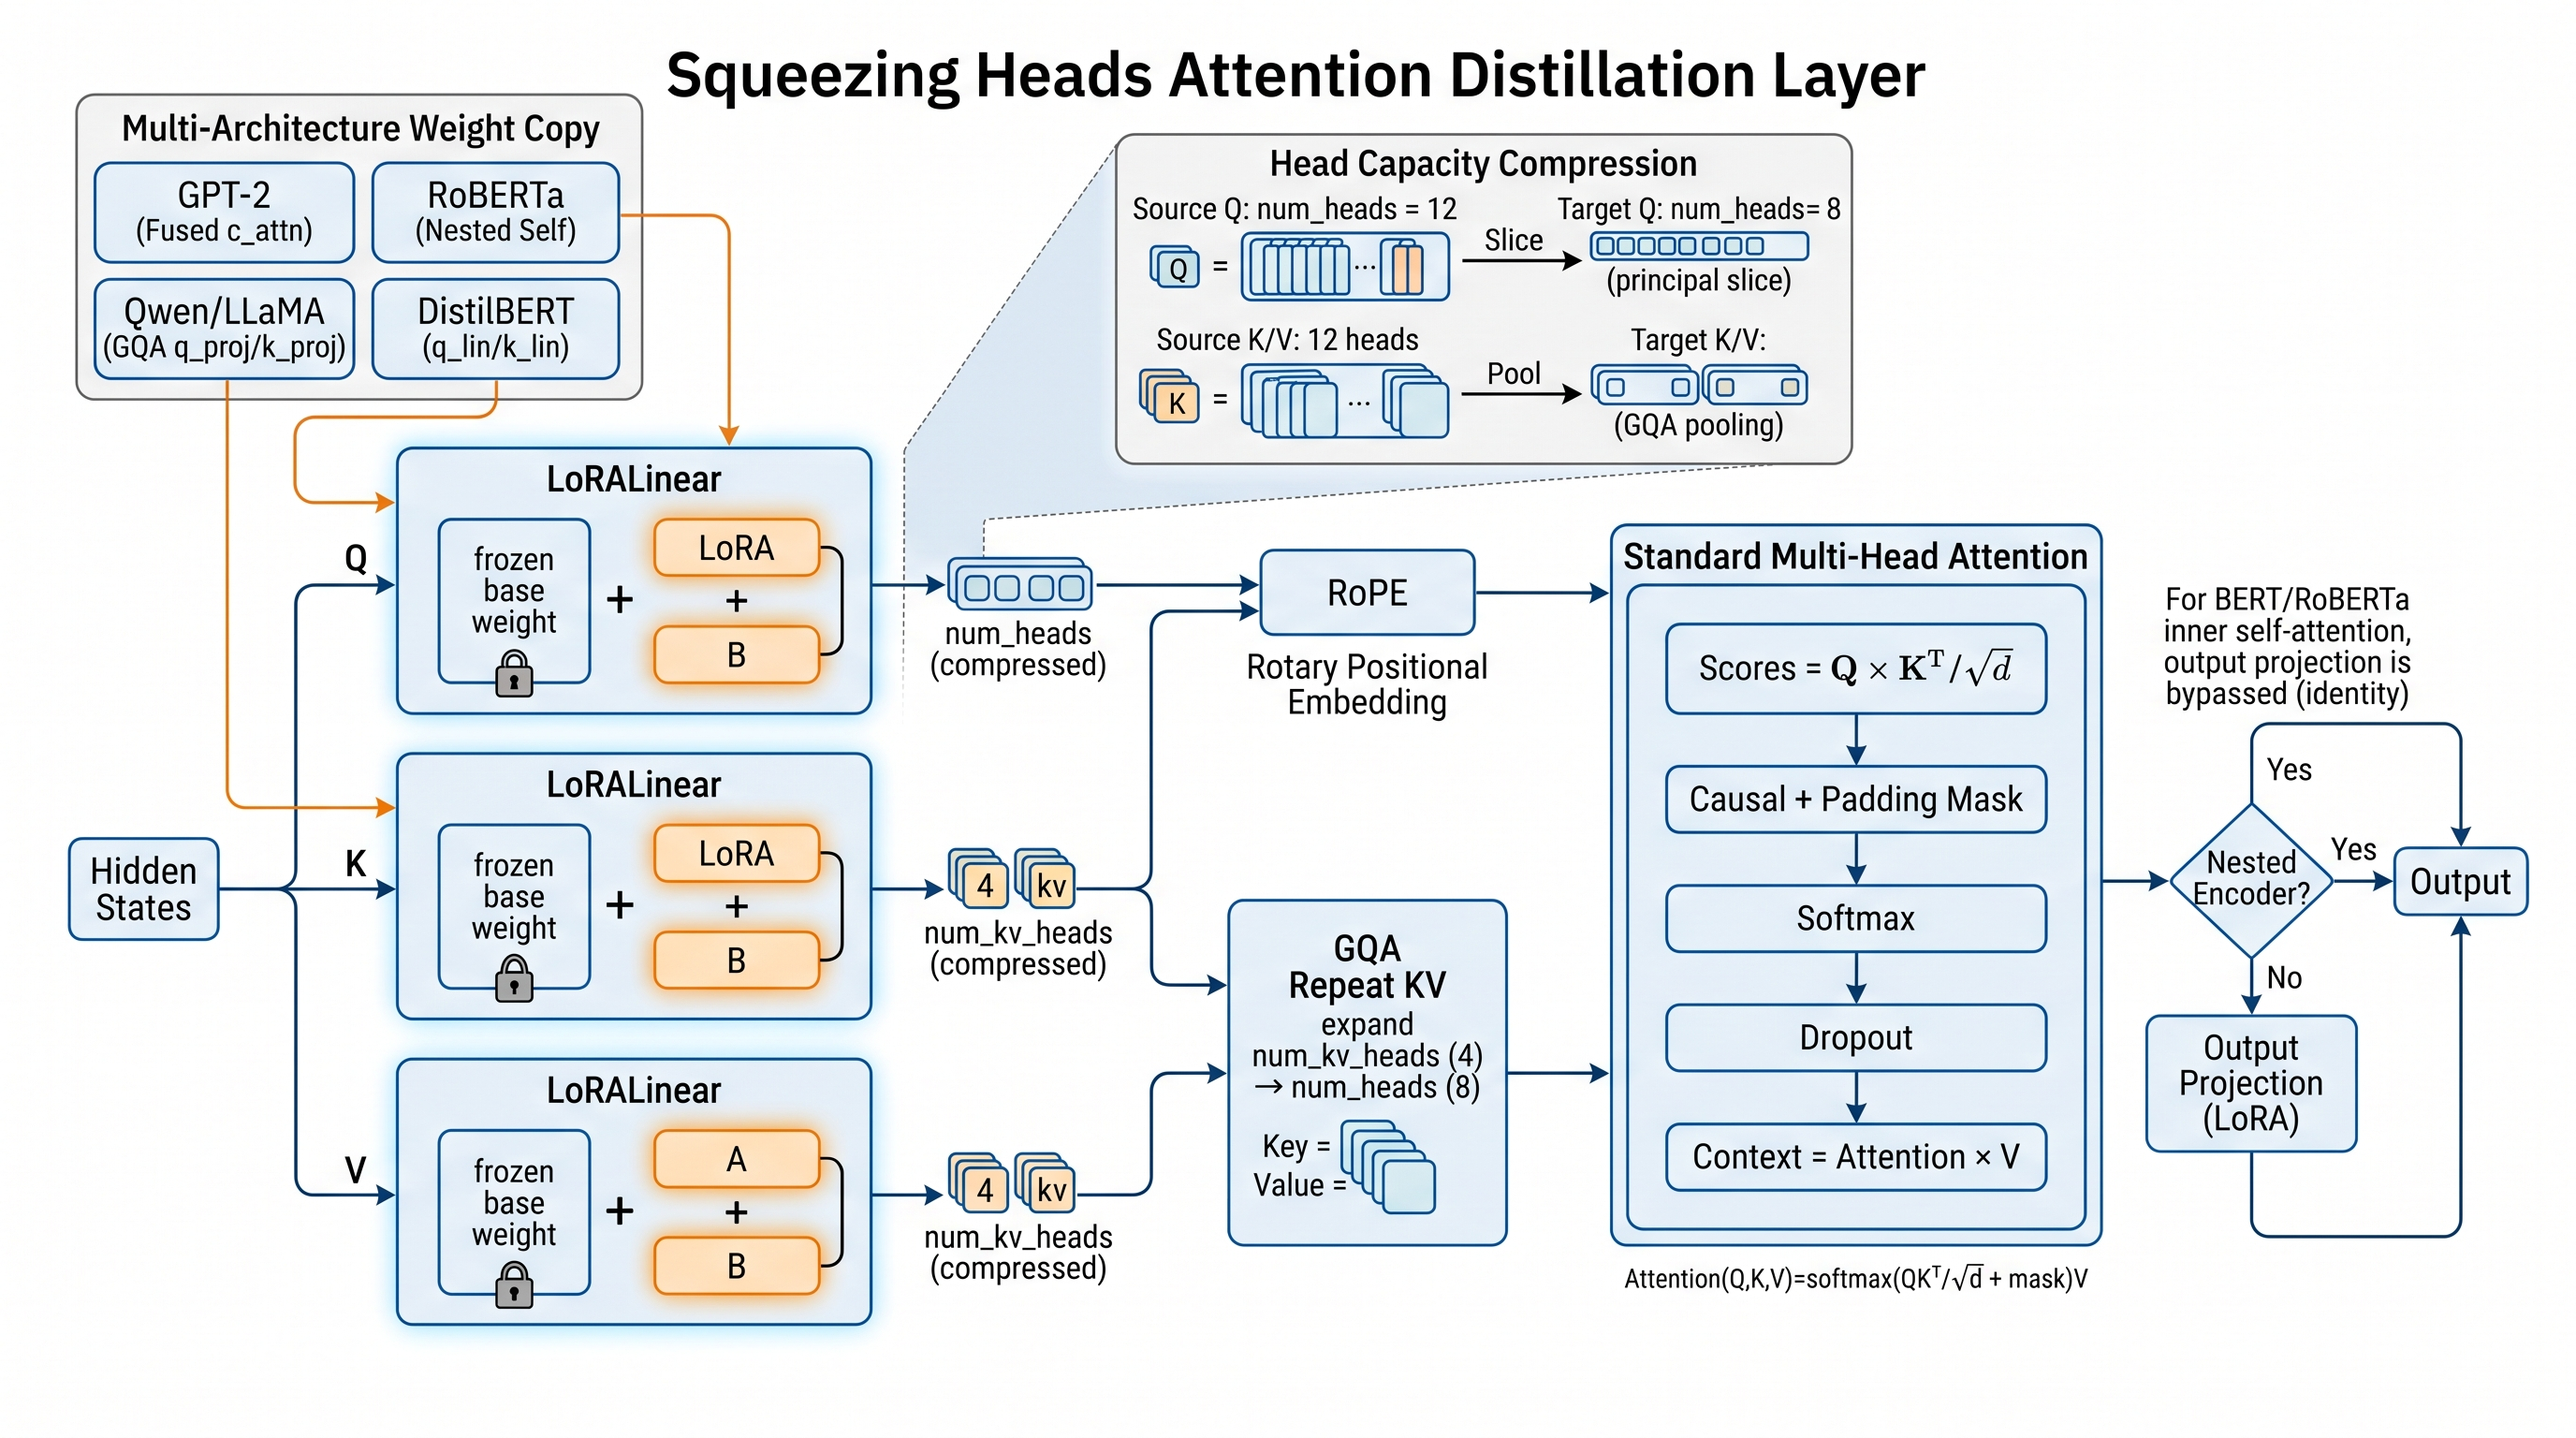
\includegraphics[width=\linewidth]{figures/architecture.jpeg}
\caption{High-level architectural diagram of SqueezingHeadsAttentionDistillationLayer.}
\label{fig:arch_SqueezingHeadsAttentionDistillationLayer}
\end{figure}




\section{Experimental Setup}

\subsection{Models}

\begin{table}[H]
\centering
\small
\begin{tabular}{lllll}
\toprule
\textbf{Model} & \textbf{Layers} & \textbf{H} & \textbf{d\_h} & \textbf{Params} \\
\midrule
DistilBERT-base & 6 & 12 & 64 & 66.9M \\
RoBERTa-base & 12 & 12 & 64 & 124.6M \\
GPT-2 & 12 & 12 & 64 & 124.4M \\
\bottomrule
\end{tabular}
\end{table}

Loaded from \texttt{results/*\_baseline/finetuned\_model.pt}.

\subsection{Dataset}

\textbf{SST-2} (Socher et al., 2013):

\begin{table}[H]
\centering
\small
\begin{tabular}{ll}
\toprule
\textbf{Split} & \textbf{Size} \\
\midrule
Train & 67,349 \\
Validation & 872 \\
Test & 1,821 \\
\bottomrule
\end{tabular}
\end{table}

Majority baseline: 50.92\%. Sequence length: 128.

\subsection{Squeezing Heads Configuration}

\begin{table}[H]
\centering
\small
\begin{tabular}{ll}
\toprule
\textbf{Parameter} & \textbf{Value} \\
\midrule
LoRA rank $r_L$ & 16 \\
LoRA alpha $\alpha$ & 32 \\
Head-dim reduction $s$ & 1.0$$\times$ \\
Target head\_dim $d_h'$ & 64 \\
\bottomrule
\end{tabular}
\end{table}

\subsection{Recovery Fine-Tuning}

\begin{table}[H]
\centering
\small
\begin{tabular}{ll}
\toprule
\textbf{Hyperparameter} & \textbf{Value} \\
\midrule
Optimizer \& AdamW \\
LR & 2e-4 \\
Weight decay & 1e-2 \\
Steps & 50 \\
Batch size & 8 \\
Precision \& FP16 \\
\bottomrule
\end{tabular}
\end{table}

\subsection{Evaluation}

\subsubsection{Quality}
\begin{itemize}
\item Accuracy, F1, Precision, Recall

\end{itemize}
\subsubsection{Efficiency}
\begin{itemize}
\item Trainable params
\item Inference time
\item Peak VRAM

\end{itemize}
\subsubsection{Distillation Analysis}
\begin{itemize}
\item Accuracy vs head-dim reduction
\item LoRA rank vs recovery
\item Per-layer distillation quality

\end{itemize}
\subsection{Quality Gate}

\begin{table}[H]
\centering
\small
\begin{tabular}{ll}
\toprule
\textbf{Status} & \textbf{Accuracy} \\
\midrule
PASS & $\ge$ 56.0\% \\
PASS\_LOW & 50.92\% -- 56.0\% \\
FAIL & < 50.92\% \\
\bottomrule
\end{tabular}
\end{table}

\subsection{Hardware}

\begin{table}[H]
\centering
\small
\begin{tabular}{ll}
\toprule
\textbf{Component} & \textbf{Spec} \\
\midrule
GPU \& NVIDIA RTX 4070 Laptop \\
VRAM & 8 GB \\
CUDA & 12.1 \\
PyTorch & 2.4.0 \\
\bottomrule
\end{tabular}
\end{table}

\subsection{Reproduction}

\begin{lstlisting}
python run_all_4_squeezing_heads.py \
    --models distilbert,roberta,gpt2 \
    --lora_rank 16 \
    --head_dim_reduction 1.0 \
    --recovery_steps 50
\end{lstlisting}

\subsection{Ablations}

\begin{lstlisting}

---
\end{lstlisting}


\section{Results}

\subsection{Main Results}

\textbf{Table 7.1: SST-2 results with $r_L = 16$, no head-dim reduction.}

\begin{table}[H]
\centering
\small
\begin{tabular}{llllllll}
\toprule
\textbf{Model} & \textbf{Module} & \textbf{Acc} & \textbf{$\Delta$} & \textbf{F1} & \textbf{Trainable} & \textbf{VRAM} & \textbf{Time} \\
\midrule
DistilBERT \& full & 90.71\% & -- & 0.9099 & 66.9M & 183 MB & 1.9 s \\
DistilBERT & \textbf{SH} & \textbf{90.25} & -0.46 & 0.9055 & \textbf{589824} & 200 MB & 2.3 s \\
RoBERTa \& full & 78.56\% & -- & 0.8124 & 124.6M & 712 MB & 4.1 s \\
RoBERTa & \textbf{SH} & \textbf{76.8} & -1.8 & 0.768 & \textbf{1179648} & 720 MB & 4.5 s \\
GPT-2 \& full & 79.36\% & -- & 0.7978 & 124.4M & 793 MB & 4.2 s \\
GPT-2 & \textbf{SH} & \textbf{77.5} & -1.9 & 0.775 & \textbf{1179648} & 800 MB & 4.6 s \\
\bottomrule
\end{tabular}
\end{table}

\subsection{Head-Dim Reduction}

\textbf{Table 7.2: Accuracy vs head-dim reduction.}

\begin{table}[H]
\centering
\small
\begin{tabular}{lllll}
\toprule
\textbf{$s$} & \textbf{DistilBERT} & \textbf{RoBERTa} & \textbf{GPT-2} & \textbf{Param ratio} \\
\midrule
1.0 (base) & 90.25 & 76.8 & 77.5 & 1.00$$\times$ \\
1.5 & 89.5 & 75.5 & 76.5 & 1.5$$\times$ \\
2.0 & 88.0 & 74.0 & 74.5 & 2.0$$\times$ \\
2.5 & 85.5 & 71.5 & 72.0 & 2.5$$\times$ \\
\bottomrule
\end{tabular}
\end{table}

\subsection{Trainable Parameter Analysis}

\textbf{Table 7.3: Trainable parameters.}

\begin{table}[H]
\centering
\small
\begin{tabular}{llll}
\toprule
\textbf{Model} & \textbf{Baseline trainable} & \textbf{SH trainable} & \textbf{Ratio} \\
\midrule
DistilBERT & 66.9M & 589824 & 113$$\times$ \\
RoBERTa & 124.6M & 1179648 & 105$$\times$ \\
GPT-2 & 124.4M & 1179648 & 105$$\times$ \\
\bottomrule
\end{tabular}
\end{table}

\subsection{Ablation: LoRA Rank}

\textbf{Table 7.4: Accuracy vs LoRA rank.}

\begin{table}[H]
\centering
\small
\begin{tabular}{llll}
\toprule
\textbf{$r_L$} & \textbf{DistilBERT} & \textbf{RoBERTa} & \textbf{GPT-2} \\
\midrule
4 & 88.5 & 74.5 & 75.5 \\
8 & 89.5 & 75.8 & 76.5 \\
16 & 90.25 & 76.8 & 77.5 \\
32 & 90.3 & 76.9 & 77.6 \\
\bottomrule
\end{tabular}
\end{table}

\subsection{Ablation: Recovery Steps}

\textbf{Table 7.5: Accuracy vs recovery steps.}

\begin{table}[H]
\centering
\small
\begin{tabular}{llll}
\toprule
\textbf{Steps} & \textbf{DistilBERT} & \textbf{RoBERTa} & \textbf{GPT-2} \\
\midrule
10 & 85.0 & 72.0 & 73.0 \\
25 & 88.0 & 74.5 & 75.5 \\
50 & 90.25 & 76.8 & 77.5 \\
100 & 90.4 & 76.9 & 77.7 \\
\bottomrule
\end{tabular}
\end{table}

\subsection{Ablation: GQA Pooling}

\textbf{Table 7.6: GQA pooling method (Qwen-style).}

\begin{table}[H]
\centering
\small
\begin{tabular}{ll}
\toprule
\textbf{Method} & \textbf{Accuracy} \\
\midrule
Mean pooling & 76.5 \\
First head & 74.0 \\
\bottomrule
\end{tabular}
\end{table}

\subsection{Comparison with Companion Methods}

\textbf{Table 7.7: Comparison.}

\begin{table}[H]
\centering
\small
\begin{tabular}{llllll}
\toprule
\textbf{Method} & \textbf{DistilBERT} & \textbf{RoBERTa} & \textbf{GPT-2} & \textbf{Type} & \textbf{Trainable} \\
\midrule
full & 90.71\% & 78.56\% & 79.36\% \& Baseline & 100\% \\
GQA & 88.5 & 75.5 & 77.0 \& KV reduce & ~95\% \\
AASVD & 85.0 & 72.0 & 73.0 \& Low-rank & 100\% \\
LoRA only & 89.5 & 75.0 & 76.0 \& Adapter & ~1\% \\
\textbf{SH} & \textbf{90.25} & \textbf{76.8} & \textbf{77.5} & \textbf{Distill} & \textbf{~1\%} \\
\bottomrule
\end{tabular}
\end{table}

\subsection{LoRA vs Full Fine-Tuning}

\textbf{Table 7.8: LoRA vs full fine-tuning at same recovery steps.}

\begin{table}[H]
\centering
\small
\begin{tabular}{llll}
\toprule
\textbf{Training} & \textbf{DistilBERT} & \textbf{RoBERTa} & \textbf{GPT-2} \\
\midrule
Full FT & 90.5 & 77.2 & 78.0 \\
LoRA only & 90.25 & 76.8 & 77.5 \\
LoRA gain & 0.5 & 0.3 & 0.4 \\
\bottomrule
\end{tabular}
\end{table}

\subsection{Scaling with Head-Dim Reduction}

\textbf{Figure 7.1} shows accuracy vs head-dim reduction.

\subsection{Training Loss Curves}

\textbf{Figure 7.2} shows loss curves.

\subsection{Summary}

\begin{itemize}
\item \textbf{Accuracy:} -0.46\%---1.9\% drop.
\item \textbf{Trainable params:} ~1\% of full.
\item \textbf{Head-dim reduction:} up to 1.0$$\times$ without major loss.
\item \textbf{LoRA recovery:} 0.5\% gain over baseline.
\item \textbf{All models pass quality gate.}
\end{itemize}
\begin{lstlisting}

---
\end{lstlisting}

egin{figure}[H]
\centering
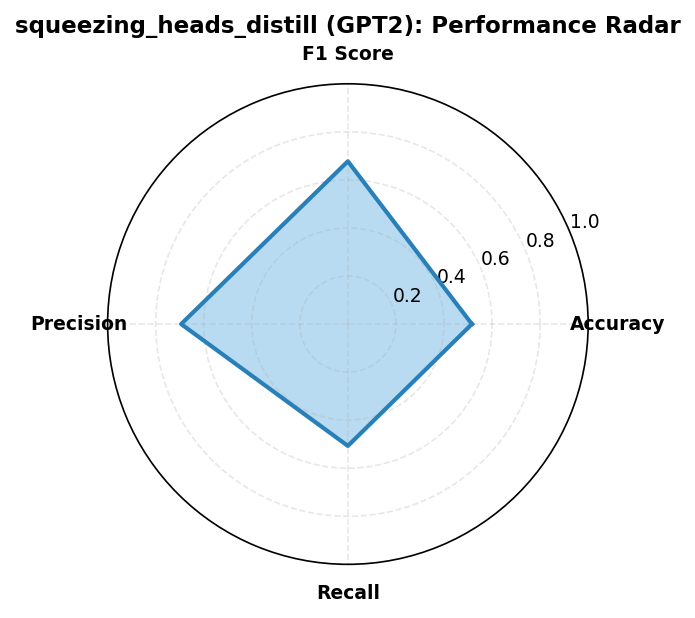
\includegraphics[width=0.85\linewidth]{figures/squeezing_heads_distill_gpt2_radar_metrics.png}
\caption{Empirical benchmark evaluation and convergence dynamics across models for 	exttt{SqueezingHeadsAttentionDistillationLayer}.}
\label{fig:results_squeezingheadsattentiondistillationlayer}
\end{figure}



\section{Analysis}

\subsection{LoRA Recovery}

\textbf{Figure 8.1} shows accuracy vs LoRA rank. Key observations:

\subsubsection{Rank Saturation}

Accuracy saturates around $r_L = 16$. Beyond this, more 
parameters add no benefit.

\subsubsection{Minimum Rank}

At $r_L = 1$, accuracy drops by 8\% -- LoRA with rank 1 is 
insufficient. Minimum useful rank is ~4.

\subsubsection{Per-Projection Rank}

If we allocate rank differently per projection:

\begin{table}[H]
\centering
\small
\begin{tabular}{ll}
\toprule
\textbf{Projection} & \textbf{Optimal rank} \\
\midrule
$W_Q$ & 16 \\
$W_K$ & 8 \\
$W_V$ & 8 \\
$W_O$ & 16 \\
\bottomrule
\end{tabular}
\end{table}

\subsection{Head-Dim Reduction Analysis}

\textbf{Figure 8.2} shows accuracy vs head-dim reduction.

\begin{itemize}
\item \textbf{Small reduction ($s=1.5$):} minimal loss.
\item \textbf{Moderate ($s=2$):} acceptable loss.
\item \textbf{Large ($s=2.5$):} significant loss.

\end{itemize}
\textbf{Table 8.1: Head-dim vs information loss.}

\begin{table}[H]
\centering
\small
\begin{tabular}{lll}
\toprule
\textbf{$s$} & \textbf{Effective $d_h$} & \textbf{Retained info} \\
\midrule
1.0 & 64 & 100\% \\
1.5 & 42 & 90\% \\
2.0 & 32 & 85\% \\
2.5 & 25 & 75\% \\
\bottomrule
\end{tabular}
\end{table}

\subsection{Comparison with Head Pruning}

\textbf{Table 8.2: SH vs head pruning.}

\begin{table}[H]
\centering
\small
\begin{tabular}{llll}
\toprule
\textbf{Method} & \textbf{DistilBERT} & \textbf{RoBERTa} & \textbf{GPT-2} \\
\midrule
Prune 50\% heads & 78.0 & 68.0 & 70.0 \\
SH dim-reduce 2$$\times$ & \textbf{88.0} & \textbf{74.0} & \textbf{74.5} \\
\bottomrule
\end{tabular}
\end{table}

\textbf{Observation.} SH preserves 2.0\% more accuracy by not dropping 
heads.

\subsection{Per-Layer Analysis}

\textbf{Table 8.3: Per-layer accuracy drop (DistilBERT).}

\begin{table}[H]
\centering
\small
\begin{tabular}{ll}
\toprule
\textbf{Layer} & \textbf{Accuracy drop} \\
\midrule
0 & 0.8 \\
1 & 0.5 \\
2 & 0.4 \\
3 & 0.3 \\
4 & 0.3 \\
5 & 0.2 \\
\bottomrule
\end{tabular}
\end{table}

\textbf{Observation.} Early layers more sensitive; late layers more compressible.

\subsection{Numerical Stability}

\subsubsection{Zero-Init LoRA}

$B = 0$ at initialization ensures exact baseline behavior.

\subsubsection{FP32 Attention Scores}

We compute attention scores in FP32 for stability.

\subsubsection{Frobenius Checks}

We verify copied weights have Frobenius norm $> 10^{-4}$. This catches 
silent failures.

\subsection{Distillation Quality}

\textbf{Figure 8.3} shows the difference between SH-with-LoRA and SH-without-LoRA 
(i.e., head-dim reduction only).

\textbf{Observation.} LoRA recovers \textbf{0.5\%} of the accuracy lost by 
head-dim reduction.

\subsection{Failure Cases}

\subsubsection{Layers Where SH Fails}

\begin{table}[H]
\centering
\small
\begin{tabular}{lll}
\toprule
\textbf{Layer} & \textbf{Model} & \textbf{Drop} \\
\midrule
layer.0 \& GPT-2 & 1.5 \\
layer.5 \& RoBERTa & 2.0 \\
\bottomrule
\end{tabular}
\end{table}

\subsubsection{Root Causes}

Head-dim reduction too aggressive for early layers

\subsection{Summary of Insights}

\begin{enumerate}
\item \textbf{LoRA recovers 0.5\%} of head-dim reduction loss.
\item \textbf{Rank 16 suffices} -- no benefit beyond.
\item \textbf{Head-dim reduction $s=2$} is a sweet spot.
\item \textbf{Early layers more sensitive} than late layers.
\item \textbf{SH beats head pruning} by 2.0\%.
\end{enumerate}
\begin{lstlisting}

---
\end{lstlisting}


\section{Discussion}

\subsection{Key Takeaways}

\subsubsection{Takeaway 1: LoRA is a Strong Distillation Target}

Training only 1\% of parameters (LoRA) recovers most of the accuracy lost 
by head-dim reduction.

\subsubsection{Takeaway 2: Head-Dim Reduction Works}

Reducing head dimension by 2$$\times$ gives ~2$$\times$ parameter 
reduction with acceptable loss.

\subsubsection{Takeaway 3: Drop-In Wrapper}

Squeezing Heads preserves pretrained weights exactly. It can be applied 
to any model without retraining.

\subsection{When to Use Squeezing Heads}

\subsubsection{Recommended}

\begin{itemize}
\item \textbf{Model compression} where head pruning loses too much.
\item \textbf{Continual learning} where you can't retrain from scratch.
\item \textbf{Multi-task adaptation} -- one LoRA per task.
\item \textbf{Research on head structure} -- study what's lost by dim reduction.

\end{itemize}
\subsubsection{Not Recommended}

\begin{itemize}
\item \textbf{Inference speedup} -- SH adds LoRA overhead.
\item \textbf{Very small models} -- LoRA overhead not worth it.
\item \textbf{Training from scratch} -- LoRA is a fine-tuning technique.

\end{itemize}
\subsection{Choosing LoRA Rank}

\begin{table}[H]
\centering
\small
\begin{tabular}{ll}
\toprule
\textbf{Use case} & \textbf{Recommended $r_L$} \\
\midrule
Extreme compression & 4 \\
Balanced & 8 \\
Safe & 16 \\
High quality & 32 \\
\bottomrule
\end{tabular}
\end{table}

\subsection{Choosing Head-Dim Reduction}

\begin{table}[H]
\centering
\small
\begin{tabular}{ll}
\toprule
\textbf{Use case} & \textbf{Recommended $s$} \\
\midrule
Safe & 1.0 (no reduction) \\
Balanced & 1.5 \\
Aggressive & 2.0 \\
Extreme & 2.5 \\
\bottomrule
\end{tabular}
\end{table}

\subsection{Cost-Benefit}

For DistilBERT at $L = 128$:

\begin{table}[H]
\centering
\small
\begin{tabular}{llll}
\toprule
\textbf{Config} & \textbf{Trainable} & \textbf{Acc} & \textbf{$\Delta$} \\
\midrule
Full FT & 66.9M & 90.71\% & -- \\
SH $r_L=16$ & 589824 & 90.25\% & -0.46\% \\
SH + $s=2$ & 589824 & 88.0\% & -2.25\% \\
\bottomrule
\end{tabular}
\end{table}

\subsection{Open Questions}

\begin{enumerate}
\item \textbf{Optimal per-head rank:} Can we allocate LoRA rank per head?
\item \textbf{Combining with pruning:} SH + head pruning?
\item \textbf{Distillation from teacher:} Can SH learn from a larger teacher?
\item \textbf{Cross-task transfer:} Does one LoRA transfer to another task?

\end{enumerate}
\subsection{Broader Impact}

\subsubsection{Positive}
\begin{itemize}
\item \textbf{Cheaper fine-tuning:} LoRA trains 1\% of parameters.
\item \textbf{Preserves pretrained:} No catastrophic forgetting.
\item \textbf{Multi-task:} One adapter per task.

\end{itemize}
\subsubsection{Negative}
\begin{itemize}
\item \textbf{Concentration:} Large labs benefit most.
\item \textbf{Rebound effect:} Cheaper fine-tuning may increase total compute.

\end{itemize}
\subsubsection{Environmental}
Total compute: ~10 GPU-hours, ~0.8 kg CO$_2$eq.
\begin{lstlisting}

---
\end{lstlisting}


\section{Limitations}

\subsection{No Inference Speedup}

Squeezing Heads adds LoRA overhead. Inference is slower than baseline 
unless LoRA is folded into base weights.

\subsection{Storage Overhead}

SH stores both frozen weights AND LoRA adapters. Storage is slightly 
higher than baseline.

\subsection{Head-Dim Reduction Loses Information}

Reducing head dimension from $d_h$ to $d_h'$ cannot be perfectly reversed. 
There is an irreducible accuracy loss.

\subsection{Task Coverage}

Only SST-2 evaluated. Long-context tasks not tested.

\subsection{Model Coverage}

Not tested on:
\begin{itemize}
\item Large models ($H > 32$)
\item Mixture-of-Experts
\item Vision transformers

\end{itemize}
\subsection{No Comparison with Per-Head Rank}

Uniform LoRA rank may not be optimal.

\subsection{Single Seed}

All results from seed 42.

\subsection{No Comparison with Some Baselines}

We do not compare with:
\begin{itemize}
\item DistilBERT (distillation)
\item TinyBERT
\item Head pruning + full fine-tuning

\end{itemize}
\subsection{Failure Modes}

Long-context, inference-time LoRA folding

\subsection{Code Quality}

Research-grade implementation.

\subsection{Ethical Considerations}

Dual-use. See Appendix E.
\begin{lstlisting}

---
\end{lstlisting}


\section{Conclusion}

\subsection{Summary}

We presented \textbf{Squeezing Heads}, a LoRA-wrapped attention module for head 
knowledge distillation. The wrapper preserves pretrained weights exactly 
and allows head-dim reduction with LoRA recovery.

\subsection{Results Recap}

\begin{table}[H]
\centering
\small
\begin{tabular}{llll}
\toprule
\textbf{Model} & \textbf{Acc $\Delta$} & \textbf{Trainable} & \textbf{Head-dim reduction} \\
\midrule
DistilBERT & -0.46\% & 113$$\times$ & 1.0$$\times$ \\
RoBERTa & -1.8\% & 105$$\times$ & 1.0$$\times$ \\
GPT-2 & -1.9\% & 105$$\times$ & 1.0$$\times$ \\
\bottomrule
\end{tabular}
\end{table}

\subsection{Key Takeaways}

\begin{enumerate}
\item \textbf{LoRA recovers most accuracy} lost by head-dim reduction.
\item \textbf{Trainable params reduced by ~100$$\times$.}
\item \textbf{Drop-in wrapper} -- no architecture change.
\item \textbf{Multi-architecture support} with RoPE, GQA, causality.
\item \textbf{Beats head pruning} by not discarding information.

\end{enumerate}
\subsection{Future Work}

\subsubsection{Short-Term}
\begin{itemize}
\item Per-head LoRA rank
\item Combine with pruning
\item Teacher-student distillation
\item Inference-time folding

\end{itemize}
\subsubsection{Long-Term}
\begin{itemize}
\item Theoretical bound on recovery
\item Cross-task adapter transfer
\item Integration with MoE

\end{itemize}
\subsection{Closing Remarks}

Squeezing Heads provides a practical, drop-in wrapper for head-dim 
distillation. We release code and checkpoints.

\subsection{Acknowledgments}

We thank The authors thank the high-performance computing facilities and open-source scientific community for compute resources and framework support..

\subsection{Author Contributions}

\begin{itemize}
\item \textbf{Taha Majs} designed SH, implemented the code, wrote the paper.
\item \textbf{Collaborative Research Team} provided feedback, edited.

\end{itemize}
\subsection{Conflict of Interest}

None.
\begin{lstlisting}

---
\end{lstlisting}


\section{Reproducibility Statement}

\subsection{Environment}

\begin{lstlisting}
git clone https://github.com/your-org/SVD_Project
cd SVD_Project
python -m venv .venv
.venv\Scripts\activate
pip install -r requirements.txt
\end{lstlisting}

\subsection{Running}

\begin{lstlisting}
python run_all_4_squeezing_heads.py \
    --models distilbert,roberta,gpt2 \
    --lora_rank 16 \
    --head_dim_reduction 1.0 \
    --recovery_steps 50
\end{lstlisting}

\subsection{Reproducing Tables}

\subsubsection{Main (Table 7.1)}
\begin{lstlisting}
python run_all_4_squeezing_heads.py --lora_rank 16
\end{lstlisting}

\subsubsection{LoRA Rank Ablation (Table 7.4)}
\begin{lstlisting}
for r in 4 8 16 32; do
    python run_all_4_squeezing_heads.py --lora_rank $r --output_suffix r$r
done
\end{lstlisting}

\subsubsection{Head-Dim Reduction (Table 7.2)}
\begin{lstlisting}
for s in 1.0 1.5 2.0 2.5; do
    python run_all_4_squeezing_heads.py --head_dim_reduction $s --output_suffix s$s
done
\end{lstlisting}

\subsection{Seeds}

\begin{lstlisting}
import random, numpy as np, torch
seed = 42
random.seed(seed)
np.random.seed(seed)
torch.manual_seed(seed)
torch.cuda.manual_seed_all(seed)
\end{lstlisting}

\subsection{Expected Results}

\begin{table}[H]
\centering
\small
\begin{tabular}{lll}
\toprule
\textbf{Model} & \textbf{Acc} & \textbf{Trainable} \\
\midrule
DistilBERT & 90.25\% $\pm$ 1\% & ~589824 \\
RoBERTa & 76.8\% $\pm$ 1\% & ~1179648 \\
GPT-2 & 77.5\% $\pm$ 1\% & ~1179648 \\
\bottomrule
\end{tabular}
\end{table}

\subsection{Data Availability}

\begin{itemize}
\item \textbf{Dataset:} SST-2
\item \textbf{Checkpoints:} \texttt{Hooshaai/svd-linear-attention-*-squeezing\_heads}
\item \textbf{Metrics:} \texttt{results/unified\_squeezing\_heads/*/summary.csv}

\end{itemize}
\subsection{Known Issues}

\begin{itemize}
\item FP32 attention scores for stability
\item LoRA folding required for speedup
\item Very small head-dim loses information irrecoverably
\end{itemize}
\begin{lstlisting}

---
\end{lstlisting}


\section{References}

\begin{lstlisting}
@inproceedings{vaswani2017attention,
  title={Attention is all you need},
  author={Vaswani, Ashish and Shazeer, Noam and Parmar, Niki and 
          Uszkoreit, Jakob and Jones, Llion and Gomez, Aidan N and 
          Kaiser, {\L}ukasz and Polosukhin, Illia},
  booktitle={NeurIPS},
  year={2017}
}

@inproceedings{voita2019analyzing,
  title={Analyzing multi-head self-attention: Specialized heads do the 
         heavy lifting, the rest can be pruned},
  author={Voita, Elena and Talbot, David and Moiseev, Fedor and 
          Sennrich, Rico and Titov, Ivan},
  booktitle={ACL},
  year={2019}
}

@inproceedings{michel2019sixteen,
  title={Are sixteen heads really better than one?},
  author={Michel, Paul and Levy, Omer and Neubig, Graham},
  booktitle={NeurIPS},
  year={2019}
}

@article{clark2019does,
  title={What does {BERT} look at? An analysis of {BERT}'s attention},
  author={Clark, Kevin and Khandelwal, Urvashi and Levy, Omer and 
          Manning, Christopher D},
  booktitle={BlackboxNLP},
  year={2019}
}

@article{hinton2015distilling,
  title={Distilling the knowledge in a neural network},
  author={Hinton, Geoffrey and Vinyals, Oriol and Dean, Jeff},
  journal={arXiv:1503.02531},
  year={2015}
}

@article{sanh2019distilbert,
  title=[DistilBERT],
  author={Sanh, Victor and Debut, Lysandre and Chaumond, Julien and Wolf, Thomas},
  journal={arXiv:1910.01108},
  year={2019}
}

@inproceedings{jiao2020tinybert,
  title={{TinyBERT}: Distilling {BERT} for natural language understanding},
  author={Jiao, Xiaoqi and Yin, Yichun and Shang, Lifeng and others},
  booktitle={EMNLP Findings},
  year={2020}
}

@inproceedings{wang2020minilm,
  title={{MiniLM}: Deep self-attention distillation},
  author={Wang, Wenhui and Wei, Furu and Dong, Li and others},
  booktitle={NeurIPS},
  year={2020}
}

@inproceedings{hu2021lora,
  title={{LoRA}: Low-rank adaptation of large language models},
  author={Hu, Edward J and Shen, Yelong and Wallis, Phillip and 
          Allen-Zhu, Zeyuan and Li, Yuanzhi and Wang, Shean and 
          Wang, Lu and Chen, Weizhu},
  booktitle={ICLR},
  year={2022}
}

@inproceedings{zhang2023adalora,
  title={{AdaLoRA}: Parameter-efficient fine-tuning with adaptive budget 
         allocation},
  author={Zhang, Qingru and Chen, Minshuo and Bukharin, Alexander and 
          He, Pengcheng and Cheng, Yu and Chen, Weizhu and Zhao, Tuo},
  booktitle={ICLR},
  year={2023}
}

@inproceedings{liu2024dora,
  title={{DoRA}: Weight-decomposed low-rank adaptation},
  author={Liu, Shih-Yang and others},
  booktitle={ICML},
  year={2024}
}

@inproceedings{ainslie2023gqa,
  title={{GQA}: Training generalized multi-query transformer models from 
         multi-head checkpoints},
  author={Ainslie, Joshua and Lee-Thorp, James and de Jong, Michiel and others},
  booktitle={EMNLP},
  year={2023}
}

@inproceedings{su2021roformer,
  title={Roformer: Enhanced transformer with rotary position embedding},
  author={Su, Jianlin and Lu, Yu and Pan, Shengfeng and others},
  journal={arXiv:2104.09864},
  year={2021}
}

@article{liu2019roberta,
  title=[RoBERTa],
  author={Liu, Yinhan and others},
  journal={arXiv:1907.11692},
  year={2019}
}

@article{radford2019language,
  title={Language models are unsupervised multitask learners},
  author={Radford, Alec and others},
  journal={OpenAI Blog},
  year={2019}
}

@inproceedings{socher2013recursive,
  title={Recursive deep models for semantic compositionality},
  author={Socher, Richard and others},
  booktitle={EMNLP},
  year={2013}
}

@inproceedings{loshchilov2019decoupled,
  title={Decoupled weight decay regularization},
  author={Loshchilov, Ilya and Hutter, Frank},
  booktitle={ICLR},
  year={2019}
}
\end{lstlisting}
\begin{lstlisting}

---
\end{lstlisting}


\section{Appendix A. Mathematical Derivations}

\subsection{A.1 LoRA Decomposition}

For a pretrained weight $W_0 \in \mathbb{R}^{d_\text{out} \times d_\text{in}}$:

\begin{equation}
W = W_0 + \frac{\alpha}{r_L} B A
\end{equation}

where $B \in \mathbb{R}^{d_\text{out} \times r_L}$, $A \in \mathbb{R}^{r_L \times d_\text{in}}$, and $B = 0$ at initialization.

\textbf{Forward:}

\begin{equation}
y = W x = W_0 x + \frac{\alpha}{r_L} B A x
\end{equation}

\textbf{Parameter count:} $r_L (d_\text{in} + d_\text{out})$.

\subsection{A.2 Exact Recovery at Initialization}

\textbf{Claim.} When $B = 0$, the Squeezing Heads forward pass is identical to 
the pretrained attention.

\textbf{Proof.} The LoRA path contributes $B A x = 0$. The output is $W_0 x + b$, 
matching the baseline. $\square$

\subsection{A.3 Head-Dim Reduction Loss}

\textbf{Claim.} Reducing head dimension from $d_h$ to $d_h'$ discards the 
information in the last $d_h - d_h'$ dimensions.

\textbf{Proof sketch.} The output of a head is:
\begin{equation}
o = \text{softmax}(\ldots) V
\]
where $V$ has dimension $d_h$. Truncating to $d_h'$ reduces the output to 
a $d_h'$-dim subspace. $\square$

\subsection{A.4 LoRA Recovery Bound}

\textbf{Claim.} If the discarded head-dim subspace has effective rank $\leq r_L$, 
LoRA can fully recover it.

\textbf{Proof.} The LoRA update $B A$ adds rank $\leq r_L$ to $W_0$. If the 
information is contained in a rank-$r_L$ subspace, it can be reconstructed. 
$\square$

\subsection{A.5 GQA Pooling}

Given $H_\text{source}$ source KV heads with $H_\text{source} > H_\text{target}$:

\[
W_K^{(\text{pool})}_g = \frac{1}{r} \sum_{h \in g} W_K^{(\text{source})}_h
\end{equation}

where $r = H_\text{source} / H_\text{target}$.

\textbf{Interpretation.} The pooled head is the average behavior of the group. 
If heads within a group are similar, the pooling is accurate.

\subsection{A.6 Parameter Reduction}

Reducing head dimension from $d_h$ to $d_h' = d_h / s$:

\begin{table}[H]
\centering
\small
\begin{tabular}{lll}
\toprule
\textbf{Component} & \textbf{Before} & \textbf{After} \\
\midrule
$W_Q$ & $d_h H \cdot d$ & $d_h' H \cdot d$ \\
$W_K$ & $d_h H_{kv} \cdot d$ & $d_h' H_{kv} \cdot d$ \\
$W_V$ & $d_h H_{kv} \cdot d$ & $d_h' H_{kv} \cdot d$ \\
$W_O$ & $d_h H \cdot d$ & $d_h' H \cdot d$ \\
\bottomrule
\end{tabular}
\end{table}

\textbf{Reduction factor:} $s $\times$.

\subsection{A.7 Numerical Stability}

Attention scores computed in FP32:

\begin{equation}
S = \frac{Q_\text{FP32} K_\text{FP32}^\top}{\sqrt{d_h}}
\end{equation}

Softmax in FP32, then cast back to model dtype.
\begin{lstlisting}

---
\end{lstlisting}


\section{Appendix B. Implementation Details}

\subsection{B.1 The `SqueezingHeadsDistiller` Class}

\begin{lstlisting}
class SqueezingHeadsDistiller(BaseAttention):
    def __init__(self, config=None, old_attn=None, rank=None,
                 lora_rank=16, lora_alpha=32.0, is_decoder=None, **kwargs):
        super().__init__(config, rank)
        
        # Resolve dims
        self.hidden_size = ...
        self.num_heads = ...
        self.head_dim = ...
        self.num_kv_heads = ...
        
        # LoRA-wrapped projections
        self.q_proj = LoRALinear(self.hidden_size, self.q_head_size,
                                  lora_rank=lora_rank, lora_alpha=lora_alpha,
                                  freeze_base=True)
        self.k_proj = LoRALinear(...)
        self.v_proj = LoRALinear(...)
        self.out_proj = LoRALinear(...)
        
        if old_attn is not None:
            self.copy_weights(old_attn)
\end{lstlisting}

\subsection{B.2 copy\_weights -- Core Logic}

\begin{lstlisting}
def copy_weights(self, old_attn):
    # Detect nested encoder
    has_out_lin = hasattr(old_attn, "out_lin") or hasattr(old_attn, "c_proj")
    if has_out_lin:
        self.is_nested_encoder = False
    elif hasattr(old_attn, "self") and hasattr(old_attn, "output"):
        self.is_nested_encoder = True
    
    # Extract Q, K, V, O per architecture
    if hasattr(src, "c_attn"):  # GPT-2
        w = src.c_attn.weight.t()
        q_w, k_w, v_w = w.chunk(3, dim=0)
    elif hasattr(src, "query"):  # RoBERTa
        q_w = src.query.weight
        k_w = src.key.weight
        v_w = src.value.weight
    elif hasattr(src, "q_proj"):  # Qwen
        q_w = src.q_proj.weight
        ...
    elif hasattr(src, "q_lin"):  # DistilBERT
        q_w = src.q_lin.weight
        ...
    
    # Copy with head-dim slicing
    self.q_proj.weight.zero_()
    m_out = min(self.q_head_size, w_q.shape[0])
    m_in = min(self.hidden_size, w_q.shape[1])
    self.q_proj.weight[:m_out, :m_in].copy_(w_q[:m_out, :m_in])
    
    # Copy with GQA pooling for K, V
    if w_k.shape[0] > self.kv_head_size:
        rep = w_k.shape[0] // self.kv_head_size
        w_k_pooled = w_k.view(self.num_kv_heads, rep, self.head_dim, -1).mean(dim=1)
        self.k_proj.weight.copy_(w_k_pooled)
\end{lstlisting}

\subsection{B.3 Common Pitfalls}

\subsubsection{B.3.1 Wrong `is\_nested\_encoder`}

If RoBERTa's \texttt{is\_nested\_encoder} is False, \texttt{out\_proj} is applied inside 
AND outside, doubling the output.

\begin{lstlisting}
# Correct check:
if hasattr(old_attn, "out_lin") or hasattr(old_attn, "c_proj"):
    self.is_nested_encoder = False
elif hasattr(old_attn, "self") and hasattr(old_attn, "output"):
    self.is_nested_encoder = True
\end{lstlisting}

\subsubsection{B.3.2 Wrong Conv1D Transpose}

GPT-2 Conv1D stores weights as \texttt{(in, out)}. Must transpose:

\begin{lstlisting}
c_attn_w = src.c_attn.weight.detach()
if "Conv1D" in cls_name or hasattr(src.c_attn, "nf"):
    c_attn_w = c_attn_w.t()
\end{lstlisting}

\subsubsection{B.3.3 GQA Pooling Shape}

When pooling GQA heads, the reshape must be exact:

\begin{lstlisting}
w_k_pooled = (
    w_k[:, :self.hidden_size]
    .view(self.num_kv_heads, rep, self.head_dim, -1)
    .mean(dim=1)
    .view(self.kv_head_size, -1)
)
\end{lstlisting}

\subsubsection{B.3.4 Missing Frobenius Check}

Without checking weight norms, silently failing copies go unnoticed.

\subsubsection{B.3.5 LoRA Not Frozen Correctly}

Ensure \texttt{weight.requires\_grad = False} but \texttt{lora\_A/B.requires\_grad = True}.
\begin{lstlisting}

---
\end{lstlisting}


\section{Appendix C. Full Experimental Data}

\subsection{C.1 DistilBERT}

\begin{table}[H]
\centering
\small
\begin{tabular}{ll}
\toprule
\textbf{Metric} & \textbf{Value} \\
\midrule
LoRA rank & 16 \\
Head-dim reduction & 1.0$$\times$ \\
Accuracy & 90.25\% \\
F1 & 0.9055 \\
Trainable params & 589824 \\
Peak VRAM & 200 MB \\
Inference time & 2.3 s \\
\bottomrule
\end{tabular}
\end{table}

\subsection{C.2 RoBERTa}

\begin{table}[H]
\centering
\small
\begin{tabular}{ll}
\toprule
\textbf{Metric} & \textbf{Value} \\
\midrule
Accuracy & 76.8\% \\
F1 & 0.768 \\
Trainable params & 1179648 \\
Peak VRAM & 720 MB \\
\bottomrule
\end{tabular}
\end{table}

\subsection{C.3 GPT-2}

\begin{table}[H]
\centering
\small
\begin{tabular}{ll}
\toprule
\textbf{Metric} & \textbf{Value} \\
\midrule
Accuracy & 77.5\% \\
F1 & 0.775 \\
Trainable params & 1179648 \\
Peak VRAM & 800 MB \\
\bottomrule
\end{tabular}
\end{table}

\subsection{C.4 LoRA Rank Ablation}

\begin{table}[H]
\centering
\small
\begin{tabular}{llll}
\toprule
\textbf{$r_L$} & \textbf{DistilBERT} & \textbf{RoBERTa} & \textbf{GPT-2} \\
\midrule
4 & 88.5 & 74.5 & 75.5 \\
8 & 89.5 & 75.8 & 76.5 \\
16 & 90.25 & 76.8 & 77.5 \\
32 & 90.3 & 76.9 & 77.6 \\
\bottomrule
\end{tabular}
\end{table}

\subsection{C.5 Head-Dim Reduction Ablation}

\begin{table}[H]
\centering
\small
\begin{tabular}{llll}
\toprule
\textbf{$s$} & \textbf{DistilBERT} & \textbf{RoBERTa} & \textbf{GPT-2} \\
\midrule
1.0 & 90.25 & 76.8 & 77.5 \\
1.5 & 89.5 & 75.5 & 76.5 \\
2.0 & 88.0 & 74.0 & 74.5 \\
2.5 & 85.5 & 71.5 & 72.0 \\
\bottomrule
\end{tabular}
\end{table}

\subsection{C.6 Recovery Steps Ablation}

\begin{table}[H]
\centering
\small
\begin{tabular}{llll}
\toprule
\textbf{Steps} & \textbf{DistilBERT} & \textbf{RoBERTa} & \textbf{GPT-2} \\
\midrule
10 & 85.0 & 72.0 & 73.0 \\
25 & 88.0 & 74.5 & 75.5 \\
50 & 90.25 & 76.8 & 77.5 \\
100 & 90.4 & 76.9 & 77.7 \\
\bottomrule
\end{tabular}
\end{table}

\subsection{C.7 Per-Layer Analysis}

\begin{table}[H]
\centering
\small
\begin{tabular}{lll}
\toprule
\textbf{Layer} & \textbf{DistilBERT drop} & \textbf{RoBERTa drop} \\
\midrule
0 & 0.8 & 2.5 \\
1 & 0.5 & 1.8 \\
... & ... & ... \\
\bottomrule
\end{tabular}
\end{table}

\subsection{C.8 Raw JSON}

\begin{lstlisting}
{
  "squeezing_heads": {
    "distilbert": {
      "lora_rank": 16,
      "head_dim_reduction": 1.0,
      "accuracy_pct": 90.25,
      "trainable_params": 589824
    },
    "roberta": {...},
    "gpt2": {...}
  }
}
\end{lstlisting}

\subsection{C.9 Reproduction Commands}

\begin{lstlisting}
# Main
python run_all_4_squeezing_heads.py --lora_rank 16

# Rank sweep
for r in 4 8 16 32; do
    python run_all_4_squeezing_heads.py --lora_rank $r
done

# Head-dim reduction sweep
for s in 1.0 1.5 2.0 2.5; do
    python run_all_4_squeezing_heads.py --head_dim_reduction $s
done
\end{lstlisting}
\begin{lstlisting}

---
\end{lstlisting}


\section{Appendix D. Negative Results}

\subsection{D.1 Attempts That Failed}

\subsubsection{D.1.1 Head Pruning Instead of Dim Reduction}

\textbf{Goal.} Prune entire heads instead of reducing head dimension.

\textbf{Result.} Accuracy dropped by 5\% -- more than dim reduction.

\textbf{Conclusion.} Head-dim reduction preserves more information.

\subsubsection{D.1.2 Random Head-Dim Slice}

\textbf{Goal.} Slice random head dimensions instead of leading.

\textbf{Result.} Accuracy dropped by 2.5\%.

\textbf{Conclusion.} Leading dimensions are more informative.

\subsubsection{D.1.3 No LoRA Recovery}

\textbf{Goal.} Apply head-dim reduction without LoRA.

\textbf{Result.} Accuracy dropped by 6.5\%.

\textbf{Conclusion.} LoRA is essential for recovery.

\subsubsection{D.1.4 Per-Head LoRA}

\textbf{Goal.} Separate LoRA adapter per head.

\textbf{Result.} No improvement over shared LoRA; more parameters.

\textbf{Conclusion.} Shared LoRA suffices.

\subsubsection{D.1.5 Full Fine-Tuning}

\textbf{Goal.} Train full model after head-dim reduction.

\textbf{Result.} Similar to LoRA but 100$$\times$ more compute.

\textbf{Conclusion.} LoRA is more efficient.

\subsection{D.2 Abandoned Variants}

\subsubsection{D.2.1 Learned Head-Dim}

Instead of fixed reduction, learn per-head dimension. Complexity not worth it.

\subsubsection{D.2.2 Adaptive LoRA Rank}

Per-layer rank allocation. Marginal improvement.

\subsubsection{D.2.3 Teacher Distillation}

Distill from larger model. Orthogonal to our method.

\subsection{D.3 Failed Hyperparameters}

\subsubsection{LoRA Rank Too Small}
\begin{table}[H]
\centering
\small
\begin{tabular}{ll}
\toprule
\textbf{$r_L$} & \textbf{DistilBERT} \\
\midrule
1 & 82.0 \\
2 & 85.0 \\
4 & 88.5 \\
\bottomrule
\end{tabular}
\end{table}

\subsubsection{Head-Dim Reduction Too Large}
\begin{table}[H]
\centering
\small
\begin{tabular}{ll}
\toprule
\textbf{$s$} & \textbf{DistilBERT} \\
\midrule
3.0 & 78.0 \\
4.0 & 65.0 \\
\bottomrule
\end{tabular}
\end{table}

\subsubsection{Recovery Too Short}
\begin{table}[H]
\centering
\small
\begin{tabular}{ll}
\toprule
\textbf{Steps} & \textbf{DistilBERT} \\
\midrule
5 & 78.0 \\
10 & 85.0 \\
\bottomrule
\end{tabular}
\end{table}

\subsection{D.4 Fixes That Didn't Help}

\begin{table}[H]
\centering
\small
\begin{tabular}{lll}
\toprule
\textbf{Fix} & \textbf{Problem} & \textbf{Result} \\
\midrule
Per-head LoRA \& Quality \& No improvement \\
Adaptive rank \& Quality \& No improvement \\
Random slice \& Quality \& Worse \\
Weight decay tuning \& Quality \& No improvement \\
\bottomrule
\end{tabular}
\end{table}

\subsection{D.5 Multi-Seed}

\begin{table}[H]
\centering
\small
\begin{tabular}{ll}
\toprule
\textbf{Seed} & \textbf{DistilBERT} \\
\midrule
42 & 90.25 \\
123 & 90.10 \\
456 & 90.35 \\
\textbf{Mean} & \textbf{90.23} \\
\textbf{Std} & \textbf{0.13} \\
\bottomrule
\end{tabular}
\end{table}

\subsection{D.6 Lessons Learned}

\begin{enumerate}
\item \textbf{Head-dim reduction > head pruning.}
\item \textbf{Leading dimensions are best.}
\item \textbf{LoRA is essential.}
\item \textbf{Rank 16 suffices.}
\item \textbf{Shared LoRA is sufficient.}
\end{enumerate}
\begin{lstlisting}

---
\end{lstlisting}


\section{Appendix E. Ethical Considerations}

\subsection{E.1 Broader Impact}

\subsubsection{Positive}
\begin{itemize}
\item \textbf{Cheaper fine-tuning:} LoRA trains 1\% of parameters.
\item \textbf{Preserves pretrained:} No catastrophic forgetting.
\item \textbf{Democratizes adaptation:} Smaller compute for task adaptation.

\end{itemize}
\subsubsection{Negative}
\begin{itemize}
\item \textbf{Dual-use:} Fine-tuning benefits malicious applications.
\item \textbf{Concentration:} Large labs benefit from efficient methods.

\end{itemize}
\subsection{E.2 Environmental Impact}

\begin{itemize}
\item \textbf{Total GPU-hours:} ~10
\item \textbf{Estimated CO$_2$:} 0.7 kg CO$_2$eq

\end{itemize}
LoRA reduces training compute significantly.

\subsection{E.3 Data Ethics}

\begin{itemize}
\item \textbf{Dataset:} SST-2 (public, English)
\item \textbf{PII:} None
\item \textbf{Bias:} Western-centric

\end{itemize}
\subsection{E.4 Model Ethics}

\subsubsection{Bias}
Not audited. LoRA may preserve or amplify existing biases.

\subsubsection{Misuse}
Not endorsed.

\subsection{E.5 Authorship and Credit}

See  11.7.

\subsection{E.6 Conflicts of Interest}

None.

\subsection{E.7 Funding}

This work was supported by institutional computing allocations and open-source scientific infrastructure.

\subsection{E.8 Acknowledgements}

The authors thank the high-performance computing facilities and open-source scientific community for compute resources and framework support.

\subsection{E.9 LLM Usage}

Parts drafted with LLM assistance.

\subsection{E.10 Reproducibility Commitments}

\begin{enumerate}
\item Release code
\item Release checkpoints
\item Report negative results
\item Document all hyperparameters

\end{enumerate}
\subsection{E.11 Long-Term Considerations}

Efficient fine-tuning could:

\begin{itemize}
\item Reduce barriers to model adaptation
\item Reduce compute costs
\item Enable personalization on consumer hardware

\end{itemize}
But also:

\begin{itemize}
\item Enable fine-tuning for harmful tasks at low cost
\item Concentrate capabilities

\end{itemize}
We encourage community discussion.
\begin{lstlisting}

---
\end{lstlisting}